\chapter{Implementações}
\label{implementa}

%\section{Algoritmos Implementados para Estudo da Convexidade $P_3$}
\section{Algoritmos Envolvendo Convexidade $P_3$}

Nesta seção apresentamos os algoritmos implementados utilizando as definições e teoremas presentes no Capítulo~\ref{cap-fundamentos}.


\subsection{Algoritmo Envoltória Convexa $P_3$}
%\subsection{Algoritmo Envolvendo Convexidade $P_3$}

O Algoritmo \ref{alg:fecho-p3} é base para os demais algoritmos,
pois os parâmetros utilizam do cálculo da envoltória convexa em suas definições.
%de problemas da convexidade $P_3$. Foi implementado 
%seguindo as definições apresentadas. 

Dado um subconjunto $S \subseteq V(G)$ de um grafo $G$.
O Algoritmo \ref{alg:fecho-p3} retorna o menor conjunto convexo $S^\prime$ de $G$ contendo $S$.
Caso $S$ seja um conjunto convexo, então o próprio $S$ é retornado.
O algoritmo utiliza a estrutura de fila (primeiro a entrar, primeiro a sair)
e as operações padrões de de inserção e remoção em fila, respectivamente $inserir()$ e $remover()$.

O Algoritmo \ref{alg:fecho-p3} utiliza $N(v)$ para representar os vértices adjacentes à $v$.
Ele utiliza também um vetor $cont[v]$, como um contador para cada vértice $v$ de $G$.

Inicialmente o Algoritmo \ref{alg:fecho-p3} enfileira os vértices de $S$ na fila e inicializa $S^\prime$ com vazio e atribui 0 a cada posição de 
\textit{cont}.

O laço das Linhas 4 a 14 implementa a função intervalo. Iterativamente, se necessário, o algoritmo inclui em $S^\prime$ novos vértices.
Quando $cont[w]$ é igual a 2, significa que w possui 2 vizinhos em $S^\prime$, então $w$ é inserido neste conjunto. 
O laço é interrompido quando a fila fica vazia.

%não serão detalhadas,
%e são relativas ações em uma estrutura de dados do tipo fila, 
%insere e remove elementos respectivamente. 

\begin{algorithm2e}
    \SetAlFnt{\tiny}
    \SetAlCapFnt{\small}
    \SetAlCapNameFnt{\small}
    \SetAlgoLined
    \DontPrintSemicolon
    \LinesNumbered
    \SetAlgoLined
    \BlankLine
    \Entrada{$G(V,E)$ e $S$ tal que $S \subseteq V(G)$}
    \Saida{$S^\prime$, menor conjunto convexo contendo $S$}
    \BlankLine

    $fila \gets S$ \\
    $S^\prime \gets \emptyset$ \\
    $cont[1...|V|] \gets 0$\\
    \Enqto{$fila \ne \emptyset$}{
        $v \gets remover(fila)$\\
        $cont[v] \gets 2$\\
        $S^\prime  \gets S^\prime \cup \{v\}$\\
        \ParaCada{$w \in N(v)$}{
            \Se{$cont[w] = 1$}{
                $inserir(w, fila)$\\
            }
            $cont[w] \gets cont[w] + 1$\\
        }
    }
\Retorna{$S^\prime$}    
\caption{$H(G(V,E),S)$}
\label{alg:fecho-p3}
\end{algorithm2e} 

%É um algoritmo polinomial, 
%em que é mantido um contador para cada vértice,
%em que cada vizinho incluído na envoltória convexa,
%é incrementado o contador. 
%Quando o contador passar de 1 para o 2, 
%o vértice será incluído na envoltória convexa,
%e seus vizinhos avaliados nas próximas iterações.

\subsection{Algoritmo Verifica Conjunto Envoltório $P_3$}
%Partindo da definição de número envoltório e do algoritmo fornecido no tópico anterior,
%a definição de um algoritmo que determine se um conjunto $S$,
%é um conjunto de envoltória, para um grafo $G$.

Trata-se de um algoritmo polinomial, 
que averigua se a envoltória convexa de um subconjunto $S \subseteq V(G)$, 
tem a mesma cardinalidade do conjunto V(G).

%\small{/* Explicar e citar a definição exata que foi utilizada */}
\begin{algorithm2e}
    \SetAlFnt{\tiny}
    \SetAlCapFnt{\small}
    \SetAlCapNameFnt{\small}
    \SetAlgoLined
    \DontPrintSemicolon
    \LinesNumbered
    \SetAlgoLined
    \BlankLine
    \Entrada{$G(V,E)$, $S \subseteq V(G)$}
    \Saida{Verdadeiro se $H(S) = V(G)$}
    \BlankLine
    $S^\prime \gets H(G(V,E),S)$ \\
    \Retorna{$|S^\prime| = |V|$} 
\caption{$ConjuntoEnvoltoria(G(V,E),S)$}
\label{alg:conjunto-envoltoria-p3}
\end{algorithm2e}

\subsection{Algoritmo Conjunto Envoltório $P_3$ de tamanho k}

Determinar se um dado grafo $G$ possui um conjunto de envoltória de tamanho k,
é um problema NP-Completo, 
conforme já visto nos fundamentos e revisão bibliográfica.

A priori a única solução exata é uma tentativa força bruta
de todas as possíveis combinações de solução.

Dessa forma o Algoritmo \ref{alg:busca-conjunto-envoltoria-p3},
reflete essa estratégia. Ele testa todos os subconjuntos de V(G) com k vértices.
Apesar de computacionalmente oneroso, demonstrou ser capaz de trazer resultados em tempo razoável, 
em grafos de até 30 vértices, conforme pode ser visto nas tabelas de resultados das próximas seções. 

No Algoritmo \ref{alg:busca-conjunto-envoltoria-p3} a função $Combinacao(V, k, i)$
retorna a combinação de vértices $V(G)$ de tamanho $k$ e índice lexicográfico $i$.
Maiores explicações sobre geração de combinações em ordem lexicográfica podem ser vistas em \cite{Itai2001}.

 \begin{algorithm2e}
    \SetAlFnt{\tiny}
    \SetAlCapFnt{\small}
    \SetAlCapNameFnt{\small}
    \SetAlgoLined
    \DontPrintSemicolon
    \LinesNumbered
    \SetAlgoLined
    \BlankLine
    \Entrada{$G(V,E)$, inteiro $k \ge 1$}
    \Saida{Verdadeiro se $G(V,E)$ tem um conjunto envoltório de tamanho k}
    \BlankLine
    $c_{nk} \gets \frac{n!}{k!(n-k)!}$\\
    \Para{i de 1 até $c_{nk}$}{
        $S \gets Combinacao(V, k, i)$\\
        \Se{$ConjuntoEnvoltoria(G(V,E),S)$}{
            \Retorna{\textbf{verdadeiro}}
        } 
    }
    \Retorna{\textbf{falso}} 
\caption{$ConjuntoEnvoltoriaK(G(V,E),k)$}
\label{alg:busca-conjunto-envoltoria-p3}
\end{algorithm2e}

Também implementamos uma versão paralela do Algoritmo \ref{alg:busca-conjunto-envoltoria-p3}.
Nesta versão são verificadas paralelamente, 
onde cada \textit{thread} trabalhadora fica responsável por um intervalo de combinações.

\subsection{Algoritmo número Envoltório $P_3$}
Sabendo-se que o número envoltório, 
é equivalente a cardinalidade do menor conjunto de envoltória de um grafo,
podemos fazer uma varredura partindo do menor conjunto possível,
até o maior possível. Ao encontrar o primeiro conjunto de envoltória,
encerra-se a busca e o tamanho desse conjunto é o número envoltório do grafo.


%\small{/* Explicar e citar a definição exata que foi utilizada */}

\begin{algorithm2e}
    %\setcounter{AlgoLine}{0}
    \SetAlFnt{\tiny}
    \SetAlCapFnt{\small}
    \SetAlCapNameFnt{\small}
    \SetAlgoLined
    \DontPrintSemicolon
    \LinesNumbered
    \SetAlgoLined
    \BlankLine
    \Entrada{$G(V,E)$}
    \Saida{h(G)}
    \BlankLine
    $h \gets 0$\\
    $k \gets 2$\\
    \Enqto{$k \le |V(G) \land h = 0$}{
        \Se{$ConjuntoEnvoltoriaK(G(V,E),k)$}{
            $h \gets k$\\
        }
        $k \gets k + 1$\\          
    }
    \Retorna{h} 
\caption{$NumeroEnvoltorio(G(V,E))$}
\label{alg:numero-envoltoria-p3}
\end{algorithm2e}

\subsection{Algoritmo heurístico Número Envoltório $P_3$}

Dado que o problema de decisão do número envoltório é NP-Completo,
obter um algoritmo heurístico pode ser viável para aplicações desse parâmetro.
Com este viés, a abordagem de um algoritmo guloso para o problema foi concebida 
nos seguintes moldes: 
\begin{itemize}
    \item{Dado um conjunto $S$ inicial, todos os vértices serão testados,
    aquele que produzir a envoltória convexa de maior cardinalidade,
    será escolhido para integrar o conjunto $S$, 
    em caso de empate o vértice com o maior grau será eleito;}
    \item{A operação se repete até que a envoltória convexa seja igual ao conjunto de vértices;}
    \item{Todos os vértices são testados como conjunto $S$ inicial;} 
    \item{Avaliar de todos os conjuntos de envoltória produzidos, 
      o resultado aproximado é a cardinalidade do menor deles.}
\end{itemize}

O algoritmo sempre encontrará um conjunto de envoltória,
porém nem sempre será o de menor cardinalidade.
A aproximação do resultado deste algoritmo será avaliada nas próximas seções.
Em que serão comparadas a aproximação de cada resultado individualmente,
categorizado por classes específicas de grafos. 

\begin{algorithm2e}
    \SetAlFnt{\tiny}
    \SetAlCapFnt{\small}
    \SetAlCapNameFnt{\small}
    \SetAlgoLined
    \DontPrintSemicolon
    \LinesNumbered
    \SetAlgoLined
    \BlankLine
    \Entrada{grafo $G(V,E)$}
    \Saida{inteiro k, número envoltório aproximado de  $G(V,E)$}
    \BlankLine

    $nenv \gets \infty $\\
    \ParaCada{$v \in V(G)$}{
        $S^\prime \gets \{v\}$\\
        $S \gets ExpandirConjuntoEnvoltoria(G(V,E),S^\prime)$\\
        $nenv \gets \min\{|S|,nenv\}$\\        
    }
    \Retorna{nenv}
\caption{$HeurísticoNEnvoltoria(G(V,E))$}
\label{alg:heurístico-numero-envoltoria-p3}
\end{algorithm2e}

 \begin{algorithm2e}
    \SetAlFnt{\tiny}
    \SetAlCapFnt{\small}
    \SetAlCapNameFnt{\small}
    \SetAlgoLined
    \DontPrintSemicolon
    \LinesNumbered
    \SetAlgoLined
    \BlankLine
    \Entrada{$G(V,E), S^\prime \subseteq V(G)$}
    \Saida{Conjunto envoltório $S^\prime$}
    \BlankLine
    \Enqto{
        $|H(G(V,E),S^\prime)| < |V(G)|$
    }{
        $ve \gets \emptyset$\\ 
        $maiorHs \gets ncve \gets 0$\\
        \ParaCada{$w \in V(G)-S^\prime$}{
            $S_{aux} \gets S^\prime \cup \{w\}$\\
            $tamHs \gets |H(G(V,E),S_{aux})|$\\
            \Se{$tamHs \ge maiorHs \land |Adj[w]| > ncve$}{
                $v_e \gets w$\\
                $maiorHs \gets tamHs$\\
                $ncve \gets  |Adj[w]| $\\
            }
        }{$S^\prime \gets S^\prime \cup \{v_e\} $}
    }
    \Retorna{$S^\prime$}
\caption{$ExpandirConjuntoEnvoltoria(G(V,E),S^\prime)$}
\label{alg:heurístico-numero-envoltoria-p3-expansao}
\end{algorithm2e}

\subsection{Algoritmo verifica Conjunto de Carathéodory $P_3$}
%A verificação se um dado conjunto $S$ é conjunto de Carathéodory $P_3$,
%é computacionalmente mais complexo que averiguar se o conjunto é de envoltória.
%Porém ainda assim, é uma verificação polinomial.

Como visto no Capítulo 2, para determinar se um certo 
subconjunto $S \subseteq V(G)$ é conjunto de Carathéodory 
basta verificar se $\partial H(S) \ne \emptyset$.

Logo o Algoritmo \ref{alg:conjunto-caratheodory-p3} simplesmente
calcula o $H(S\textbackslash u)$ para todo $u \in S \subseteq V(G)$ 
e realiza a união. Se o resultado for não vazio então $S$ é um conjunto de Carathéodory.

Para calcular $H(S\textbackslash u)$ o algoritmo utiliza o Algoritmo \ref{alg:fecho-p3} como sub-rotina.

\begin{algorithm2e}
    \SetAlFnt{\tiny}
    \SetAlCapFnt{\small}
    \SetAlCapNameFnt{\small}
    \SetAlgoLined
    \DontPrintSemicolon
    \LinesNumbered
    \SetAlgoLined
    \BlankLine
    \Entrada{$G(V,E)$, $S \subseteq V(G)$}
    \Saida{Verdadeiro se $S$ é um conjunto de Carathéodory}
    \BlankLine
    $S^\prime \gets H(G(V,E),S)$ \\
    \ParaCada{$u \in S$}{
        $S^{\prime \prime} \gets H(G(V,E),S \textbackslash \{u\})$ \\
        $S^\prime \gets S^\prime \textbackslash S^{\prime \prime}$ \\
    }
    \Retorna{$S^\prime \ne \emptyset$} 
\caption{$ConjuntoCaratheodory(G(V,E),S)$}
\label{alg:conjunto-caratheodory-p3}
\end{algorithm2e}

%Primeiramente é obtido a envoltória convexa do conjunto $S$ (linha 1).
%Depois computado a envoltória convexa de S sem cada um de seus elementos,
%removendo da envoltória convexa de S essas envoltórias parciais (linha 2-5).
%Até que finalmente é verificado se ainda existem elementos na envoltória convexa de S(linha 6), 
%ou seja o conjunto $S$ é de Carathéodory.

\subsection{Algoritmo conjunto de Carathéodory $P_3$ de tamanho k}
Tal qual determinar se $G$ tem um conjunto envoltório de tamanho k, 
determinar se um dado grafo $G$ possui um conjunto de Carathéodory de tamanho k é um problema NP-Completo.

No Algoritmo \ref{alg:busca-conjunto-caratheodory-p3},
temos uma abordagem força bruta, testando, no pior caso,
todos os subconjuntos de k vértices de V(G).
%utilizando sucessivas tentativas de possíveis combinações de solução de tamanho k. 

\begin{algorithm2e}
    \SetAlFnt{\tiny}
    \SetAlCapFnt{\small}
    \SetAlCapNameFnt{\small}
    \SetAlgoLined
    \DontPrintSemicolon
    \LinesNumbered
    \SetAlgoLined
    \BlankLine
    \Entrada{$G(V,E)$, inteiro $k \ge 1$}
    \Saida{Verdadeiro, se o grafo $G(V,E)$ tem um conjunto de Carathéodory de tamanho k}
    \BlankLine
    $c_{nk} \gets \frac{n!}{k!(n-k)!}$\\
    \Para{i de 1 até $c_{nk}$}{
        $S \gets Combinacao(V, k, i)$\\
        \Se{$ConjuntoCaratheodory(G(V,E),S)$}{
            \Retorna{\textbf{verdadeiro}}
        } 
    }
    \Retorna{\textbf{falso}} 
\caption{$ConjuntoCaratheodoryK(G(V,E),k)$}
\label{alg:busca-conjunto-caratheodory-p3}
\end{algorithm2e}

Como no Algoritmo \ref{alg:busca-conjunto-caratheodory-p3} não é um algoritmo polinomial,
uma implementação paralela foi realizada.
Todas as combinações são verificadas paralelamente,
onde cada \textit{thread} trabalhadora fica responsável
por um intervalo de combinações.

\subsection{Algoritmo Número de Carathéodory $P_3$}
Por definição, temos que o número de Carathéodory de um grafo 
é a cardinalidade do maior conjunto de Carathéodory.

A abordagem indicada então é fazer uma varredura partindo do maior até o menor conjunto possível.
Como o limite para o número de Carathéodory é $c(G) \le \frac{n(G) + 1}{2}$,
iniciamos com conjuntos deste tamanho. Também utilizamos o Algoritmo \ref{alg:busca-conjunto-caratheodory-p3}
pra testar se existe um conjunto de Carathéodory de tamanho k.
Ao encontrar o primeiro conjunto de Carathéodory, o algoritmo encerra a busca 
e o tamanho desse conjunto é o número de Carathéodory do grafo.

\begin{algorithm2e}
   \SetAlFnt{\tiny}
    \SetAlCapFnt{\small}
    \SetAlCapNameFnt{\small}
    \SetAlgoLined
    \DontPrintSemicolon
    \LinesNumbered
    \SetAlgoLined
    \BlankLine
    \Entrada{$G(V,E)$}
    \Saida{$c(G)$}
    \BlankLine
    $c \gets 0$\\
    $k \gets \frac{n + 1}{2}$\\
    \Enqto{$k \ge 1 \land c = 0$}{
        \Se{$ConjuntoCaratheodoryK(G(V,E),k)$}{
            $c \gets k$\\
        }
        $k \gets k - 1$\\ 
    }
    \Retorna{c}
\caption{$NumeroCaratheodory(G(V,E))$}
\label{alg:numero-caratheodory-p3}
\end{algorithm2e}

\subsection{Algoritmo Heurístico para o Número de Carathéodory $P_3$}

Dado que obter o número de Carathéodory é um problema NP-Completo,
uma tentativa de algoritmo heurístico para instâncias grandes e médias do problema,
seria uma opção viável para o estudo desse parâmetro.

Com este viés, a abordagem de um algoritmo guloso para o problema foi concebida em duas partes.

A primeira parte é o Algoritmo \ref{alg:heurístico-numero-caratheodory-p3-parcial} em que um conjunto de Carathéodory é construído de forma reversa,
partindo do vértice que se deseja que esteja no $\partial H(S)$,
fazendo sucessivos testes de troca de um vértice em S, 
por um par de seus vizinhos. 
O algoritmo utiliza a rotina $Adj2MenorGrau[v,C]$, que retorna os vertices $u$ e $w$,
tal que $u,w\in Adj[v] \textbackslash C$, e $u$ e $w$ possuem o menor dentre as opções.

O resultado da primeira etapa é sempre um conjunto de Carathéodory,
que será a entrada da segunda parte, o Algoritmo \ref{alg:heurístico-numero-caratheodory-p3-expansao} segue conforme: 
\begin{itemize}
    \item{Dado um conjunto de Carathéodory $S$ inicial, todos os vértices serão testados. 
    Aquele que adicionado ao conjunto inicial e produzir um conjunto de Carathéodory de menor cardinalidade,
    será escolhido para integrar o conjunto $S$. Em caso de empate o vértice com o menor grau será eleito;}
    \item{A operação se repete até que não seja possível adicionar um novo vértice e produzir um conjunto de Carathéodory;}
\end{itemize}

O algoritmo sempre encontrará um conjunto de Carathéodory,
porém nem sempre será o maior possível.
A aproximação do resultado deste algoritmo será avaliada nas próximas seções,
em que serão comparadas a aproximação de cada resultado individualmente,
categorizado por tipo de grafo. 

%\small{/* Explicar e citar a definição exata que foi utilizada */}
\begin{algorithm2e}
    \SetAlFnt{\tiny}
    \SetAlCapFnt{\small}
    \SetAlCapNameFnt{\small}
    \SetAlgoLined
    \DontPrintSemicolon
    \LinesNumbered
    \SetAlgoLined
    \BlankLine
    \Entrada{$G(V,E)$}
    \Saida{inteiro k, número aproximado de Carathéodory de  $G(V,E)$}
    \BlankLine
    $c \gets 0$\\
    \ParaCada{$v \in V(G)$ tal que $|Adj[v]| \ge 2$}{
        $S \gets ConstroiConjCaratheodoryDoParcial(G(V,E),v)$\\
        $S \gets ExpandirConjuntoCaratheodory(G(V,E),S)$\\
        $c \gets \max\{|S|,ncarat\}$\\        
    }
    \Retorna{c}
\caption{$HeurísticoNCaratheodory(G(V,E))$}
\label{alg:heurístico-numero-caratheodory-p3}
\end{algorithm2e}

%\small{/* Explicar e citar a definição exata que foi utilizada */}

 \begin{algorithm2e}
    \SetAlFnt{\tiny}
    \SetAlCapFnt{\small}
    \SetAlCapNameFnt{\small}
    \SetAlgoLined
    \DontPrintSemicolon
    \LinesNumbered
    \SetAlgoLined
    \BlankLine
    \Entrada{$G(V,E)$ e vértice $v \in V(G)$ tal que $|Adj[v]| \ge 2$}
    \Saida{conjunto de Caratheodory $S$}
    \BlankLine
    $S \gets \{v\}$\\
    $fila \gets S$ \\
    \Enqto{
        $fila \ne \emptyset$
    }{
        $v_p \gets remover(fila)$\\
        $S^\prime \gets Adj2MenorGrau[v_p,S\cup\{v\}]$\\
        $S_{aux} \gets S^\prime \cup S \textbackslash \{v_p\} $\\
        \Se{$ConjuntoCaratheodory(G(V,E),S_{aux})$}{
            $inserir(S^\prime, fila)$\\
            $S \gets S_{aux}$\\
        }
    }
    \Retorna{S}
\caption{$ConstroiConjCaratheodoryDoParcial(G(V,E),v)$}
\label{alg:heurístico-numero-caratheodory-p3-parcial}
\end{algorithm2e}

 \begin{algorithm2e}
    \SetAlFnt{\tiny}
    \SetAlCapFnt{\small}
    \SetAlCapNameFnt{\small}
    \SetAlgoLined
    \DontPrintSemicolon
    \LinesNumbered
    \SetAlgoLined
    \BlankLine
    \Entrada{$G(V,E)$}
    \Entrada{vértice $v \in V(G)$}
    \Saida{conjunto de Carathéodory S otimizado}
    \BlankLine
    \Repita{
        $V_e \ne \emptyset $
    }{
        $Ve \gets \emptyset$\\
        $t_{hsve} \gets \infty$\\
        \ParaCada{$v \in V(G) \textbackslash S$}{
            $S_{aux} \gets S \cup \{v\}$\\
            $cc \gets ConjuntoCaratheodory(G(V,E),S_{aux})$
            $t_{hs} \gets |H(G(V,E),S_{aux})|$\\
            \Se{$cc \land (t_{hsve} =  \infty \lor (t_{hs} \le t_{hsve} \land |Adj[v]| < |Adj[v_e]|))$}{
                $V_e \gets \{v\}$\\
                $t_{hsve} \gets t_{hs}$\\
            }
        }{$S \gets S \cup \{V_e\} $}
    }
    \Retorna{S}
\caption{$ExpandirConjuntoCaratheodory(G(V,E),S)$}
\label{alg:heurístico-numero-caratheodory-p3-expansao}
\end{algorithm2e}

\subsection{Otimização do Algoritmo heurístico Número Envoltório $P_3$}

Com objetivo de acelerar o processamento dos algoritmos e explorar uma maior quantidade de grafos, otimizações foram feitas no Algoritmo \ref{alg:heurístico-numero-envoltoria-p3}, utilizando estratégias de paralelismo.
Para tal, decidimos pela abordagem de processar o maior número possível de grafos pequenos e médios. Essa estratégia atendia as demandas de execução realizadas até essa etapa do trabalho. Portanto, abrimos mão da abordagem de lidar com poucos grafos grandes, apesar de serem suportados, para realizar melhorias que atendessem a execução para grafos pequenos e médios.

Para uma paralelização efetiva e com ganho de desempenho real a implementação deve levar em conta o formato dos dados de entrada, acesso aglutinado das \textit{threads} trabalhadoras, divisão do problema em pequenos trabalhos, combinação das respostas e uma alta taxa de ocupação da $GPU$.

Iniciamos por desenvolver uma forma de entrada de dados que proporcionasse um bom acesso aglutinado. Para um bom desempenho paralelo é desejável que as \textit{threads} acessem os dados de trabalho de forma aglutinada. Dentre as diversas formas de se representar a estrutura de dados de um grafo, uma bastante utilizada em implementações paralelas com grafos é a forma compacta da lista de adjacência,
ou linha de adjacência compacta. Essa estrutura de dados é conhecida como \textit{Compressed Sparse Row} (CSR)\cite{Reviewed2009,Fu2014,Merrill2012,Wang2015} e para a maioria das soluções se mostrou eficiente, do ponto de vista de uso de memória, cache e acesso a uma região uniforme de memoria. Logo, por esses motivos, essa foi a forma escolhida para a implementação neste trabalho.

\begin{figure}[h]
\centering
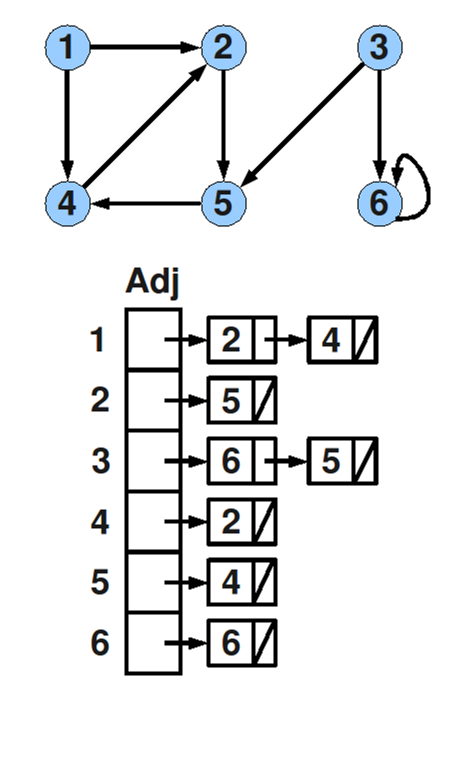
\includegraphics[width=10pc]{./imagens/adj-list-2.png}
\caption{Grafo na forma de lista de adjacência}
\label{fig_adj}
\textit{Fonte: Adaptado de \cite{nonato2000}}
\end{figure}

A representação de um grafo simples na forma CSR pode ser feita com apenas 2 vetores. Um deles contendo a concatenação em ordem de todas as listas de adjacências do grafo, e um segundo vetor contendo um índice com a posição de início da lista de adjacência de cada vértice. Uma representação visual dessa estrutura pode ser vista na Figura~\ref{fig_csr}.

\begin{figure}[h]
\centering
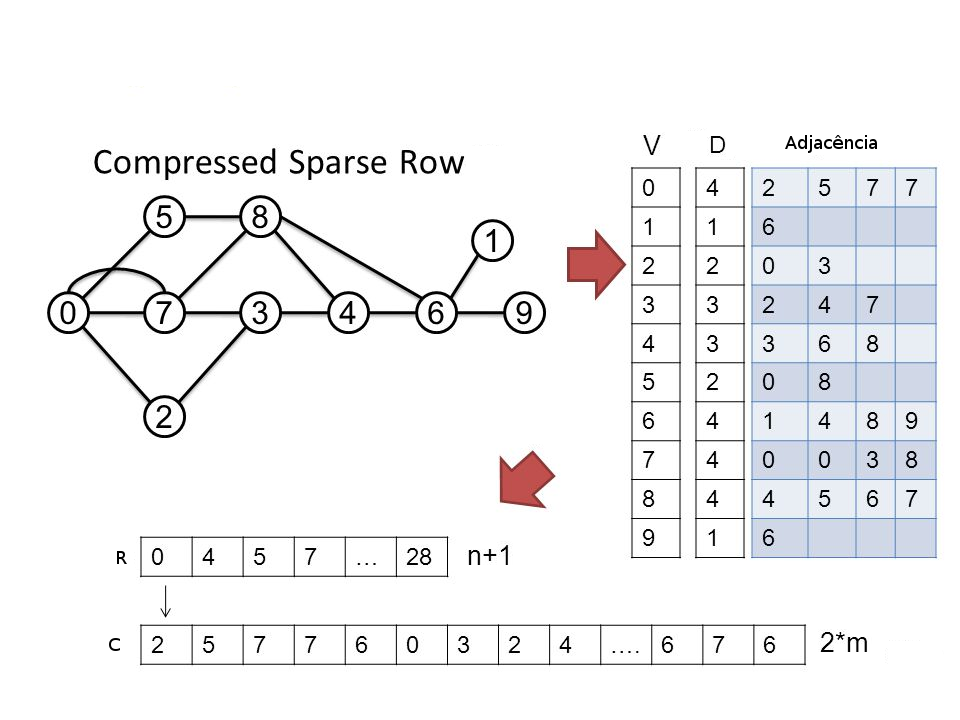
\includegraphics[width=20pc]{./imagens/csr-exemplo.png}
\caption{Grafo na forma compacta}
\label{fig_csr}
\textit{Fonte: Adaptado de \cite{kamesh2011}}     
\end{figure}


A escolha do particionamento do problema é um fator importante no incremento da performance do processamento paralelo. O ideal é uma estratégia que utilize sabiamente a quantidade de \textit{threads} existentes, de modo que o trabalho executado esteja balanceado \cite{Hong2011b,Hong2011a}. Inicialmente foram investigados três abordagens: uma \textit{thread} pra cada grafo, um bloco de \textit{threads} para cada grafo e uma \textit{thread} para cada vértice.

Analisamos essas três abordagens aplicando a grafos de até 20 vértices de um banco de grafos \cite{hog2013}. 
Após a avaliação, apesar de praticamente todas serem abordagens mais rápidas que uma implementação serial, 
até as melhores apresentaram algum tipo de gargalo em alguma etapa. Com isso, escolhemos uma combinação da abordagem de grafo/bloco com grafo/vértice  para trazer os benefícios de cada uma das abordagens, 
minimizando as possíveis ineficiências de cada. Com esse objetivo,
foi desenvolvido o Algoritmo \ref{alg-heurístico-abordagem-hibrida}, com dois núcleos. 

O primeiro núcleo, chamado de \textit{Kernel-1}, particiona o trabalho do grafo em blocos inteiros. Caso um bloco não seja totalmente utilizado, esse trabalho fracionado ficará a cargo do segundo núcleo, também chamado de \textit{Kernel-2}. Considere \textit{TAMBLOCK} a quantidade máxima de \textit{threads} ativas. Assim, o \textit{Kernel-1} trabalhará com grafos cuja a quantidade de vértices seja maior ou igual a um múltiplo do tamanho de \textit{TAMBLOCK}. O \textit{Kernel-2} agrupa o trabalho restante em blocos com tamanho múltiplo do \textit{TAMBLOCK}. 

O Algoritmo \ref{alg-heurístico-abordagem-hibrida} utiliza as abordagens grafo/bloco e vértice/\textit{thread} através dos núcleos 1 e 2 descritos anteriormente.

\begin{algorithm2e}
\SetAlFnt{\tiny}
\SetAlCapFnt{\small}
\SetAlCapNameFnt{\small}
\SetAlgoLined
\Entrada{$G_s$}
\Saida{Envoltória Aproximada de $G_s$}
\Inicio{
$ R_s \gets \emptyset $\\
$ M_w \gets \emptyset $\\
$ nblk \gets 0 $\\
$ TAMBLOCKTRUNC \gets TAMBLOCK $\\


\ParaCada{$g \in G_s$}{
  $n \gets |V(g)|$ \\
  $R_s[g] \gets n $\\
  \Se{$n \ge TAMBLOCK $}{
    $nblk \gets nblk + 1$\\
  }
  $nvtrunc \gets n$ {\bf mod} $TAMBLOCK $\\
  $tntrunc \gets tntrunc + vtrunk $\\        
  \Para{$i$ de $1$ até $nvtrunc$}{
	$v \gets \frac{n}{TAMBLOCK} \times TAMBLOCK + i$ \\
	$ M_w.add(\{g,v\})$\\
  }
}
$nblktrunc \gets \frac{nvertstrunk}{TAMBLOCKTRUNC}$\\
$kAproxEnvoltGrafBlk<<<nblk, TAMBLOCK>>>(G_s, R_s)$\\
$kAproxEnvGrafBlkTrunc<<<nblktrunc, TAMBLOCKTRUNC>>>(G_s, R_s, M_w, tntrunc)$\\
\Retorna{$R_s$}
}
\caption{HeurísticoNEnvoltorioPCombinado}
\label{alg-heurístico-abordagem-hibrida}
\end{algorithm2e}



\begin{algorithm2e}
\SetAlFnt{\tiny}
\SetAlCapFnt{\small}
\SetAlCapNameFnt{\small}
\SetAlgoLined
\Entrada{$G_s$}
\Saida{Nº Envoltório Aproximado $R_s$ }	
    $shared$ $rlocal$\\			
	\Se{$threadIdx = 0$}{
    	$rlocal \gets \infty$\\
    }
    $syncthreads()$\\
	$g \gets G_s[blockIdx]$\\
    $n \gets |V(g)|$\\
    $id \gets threadIdx$\\        
    $i \gets 0$\\
    \Enqto{
    	$id < n$
    }{
    	$v \gets id$\\
        $S^\prime \gets \{v\}$\\                                
        \Enqto{$|H(g,S^\prime)| < n$}{
            $ve \gets \emptyset$\\ 
            $mHs \gets ncve \gets 0$\\
            \ParaCada{$w \in V(g)-S^\prime$}{
                $S_{aux} \gets S^\prime \cup \{w\}$\\
                $tHs \gets |H(g,S_{aux})|$\\
                \Se{$tHs \ge mHs \land |Adj[w]| > ncve$}{
                    $v_e \gets w$\\
                    $mHs \gets tHs$\\
                    $ncve \gets  |Adj[w]| $\\
                }
            }{$S^\prime \gets S^\prime \cup \{v_e\}$}
        }
        
        $i \gets i + 1$\\
        $id \gets id + (i \times TAMBLOCK)$\\
    }
		$syncthreads()$\\
    \Se{$threadIdx = 0$}{
    	$R_s[g]=rlocal$\\
    }
\caption{kAproxEnvoltGrafBlk}
\label{alg:heurístico-numero-envoltoria-p3-mix}
\end{algorithm2e}

\begin{algorithm2e}
\SetAlFnt{\tiny}
\SetAlCapFnt{\small}
\SetAlCapNameFnt{\small}
\SetAlgoLined
\Entrada{$G_s$, $M_w$, $tntrunc$}
\Saida{Nº Envoltório Aproximado $R_s$ }
$id \gets blockIdx + threadIdx$\\
$i \gets 0$\\
\Enqto{
$id < tntrunc$
}{
$g \gets M_w[id][0]$\\
$v \gets M_w[id][1]$\\
%exapandHullSetFromV\\
$S^\prime \gets \{v\}$\\
\Enqto{$|H(g,S^\prime)| < n$}{
    $ve \gets \emptyset$\\
    $mHs \gets ncve \gets 0$\\
    \ParaCada{$w \in V(g)-S^\prime$}{
        $S_{aux} \gets S^\prime \cup \{w\}$\\
        $tHs \gets |H(g,S_{aux})|$\\
        \Se{$tHs \ge mHs \land |Adj[w]| > ncve$}{
            $v_e \gets w$\\
            $mHs \gets tHs$\\
            $ncve \gets  |Adj[w]| $\\
        }
    }{$S^\prime \gets S^\prime \cup \{v_e\}$}
}
$i \gets i + 1$\\
$id \gets id + (i \times TAMBLOCKTRUNC)$\\
$atomicMin(R_s[g],|S^\prime|)$\\
}
\caption{kAproxEnvGrafBlkTrunc}
\end{algorithm2e}



\begin{figure}[h]
\centering
\begin{tikzpicture}
  \begin{axis}
  [xlabel={Quantidade de grafos}, ylabel={Tempo(s)},legend pos=north west,axis lines=left]
  \addplot[name path=maxi,mark=none,blue] coordinates {
  (6,0) (48,10.1) (96,10.2) (384,40.1) (620,57.5) (1024,70.3) 
  };
  \addlegendentry{serial}
  
  \addplot[name path=maxi,mark=none,red] coordinates {
  (6,0) (48,303) %(96,608) %(384,0) (620,0) (1024,0) 
  };
  \addlegendentry{grafo/thread}

  \addplot[name path=maxi,mark=none,green] coordinates {
  (6,0) (48,12.5) (96,12.6) (384,15.3) (620,38.6) (1024,38.7) 
  };
  \addlegendentry{grafo/bloco}

  \addplot[name path=maxi,mark=none,yellow] coordinates {
  (6,0) (48,3.6) (96,4.3) (384,13.8) (620,37.1) (1024,37.4) 
  };
  \addlegendentry{vertice/thread}
  
  \addplot[name path=maxi,mark=none] coordinates {
  (6,0) (48,3.6) (96,13) (384,17.3) (620,37.1) (1024,38.8) 
  };
  \addlegendentry{combinada}
  \end{axis}
\end{tikzpicture}
\caption{Crescimento heurístico}
\label{fig-crescimento-num-heurístico}
\end{figure}

Com essa abordagem combinada, conseguimos melhorar os tempos de execução em pelo menos quatro vezes,
conforme podemos ver no gráfico da Figura~\ref{fig-crescimento-num-heurístico} e na Tabela~\ref{tab-speedups-paralelos}.

\begin{table}[H]
\centering
\caption{Tempo de execução das implementações aproximativas paralelas}
\label{tab-speedups-paralelos}
\begin{tabular}{l|l|l|l|l|}
\cline{2-5}
                                              & \multicolumn{4}{l|}{\textbf{Tempo em segundos de execução}}                            \\ \hline
\multicolumn{1}{|l|}{\textbf{Estrategia}}     & \textbf{100 grafos} & \textbf{300 grafos} & \textbf{600 grafos} & \textbf{1000 grafos} \\ \hline
\multicolumn{1}{|l|}{\textbf{grafo/thread}}   & 303                 & -                   & -                   & -                    \\ \hline
\multicolumn{1}{|l|}{\textbf{grafo/bloco}}    & 12.6                & 15.3                & 38.6                & 38.7                 \\ \hline
\multicolumn{1}{|l|}{\textbf{vértice/thread}} & 4.3                 & 13.8                & 37.1                & 38.4                 \\ \hline
\multicolumn{1}{|l|}{\textbf{combinada}}      & 13                  & 17.3                & 37.1                & 37.4                 \\ \hline
\end{tabular}
\end{table}


\section{Ferramenta Desenvolvida: FATIG}

Ao decorrer da execução do trabalho, uma ferramenta foi desenvolvida para facilitar a utilização dos algoritmos implementados, visualização e consulta histórica dos resultados obtidos. Apresentaremos a FATIG - {\it F}erramenta {\it A}berta para {\it T}estes e {\it I}mplementações para {\it P}roblemas em {\it G}rafos.
Apesar de não ser o objetivo do trabalho, deixaremos aqui uma visão geral de como usar e as tecnologias empregadas. 
E a quem puder interessar, estará disponível um código e um \textit{livedemo}.

%\subsection{Modo de Usar}
A FATIG pode ser acessada por qualquer navegador web. O usuário pode fornecer um arquivo com um grafo de interesse,
ou gerar um dentre os geradores disponíveis. 
Com algum grafo carregado o usuário pode executar 
qualquer problema das categorias fornecidas e
visualizar o resultado ao termino da execução. No Apêndice~\ref{apend-ferramenta},
temos figuras da tela principal da FATIG com mais detalhes.


% \begin{figure}[h]
% \begin{center}
% 	\caption{Ferramenta para Execução de Algoritmos}
%     \label{fig-ferramenta-grafo}
% 	\begin{center}
% 	    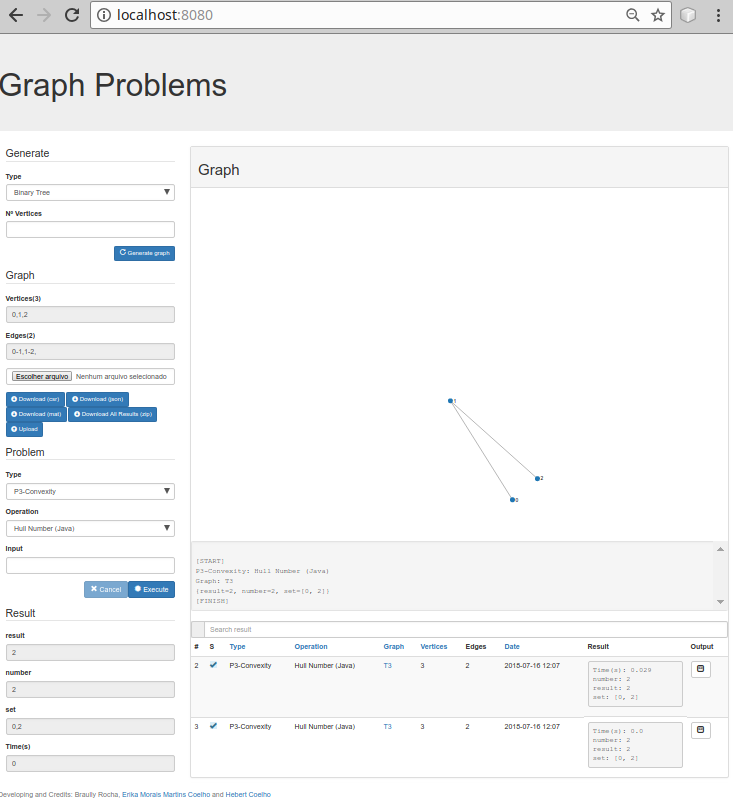
\includegraphics[width=0.8\textwidth]{./imagens/ferramenta-tela-principal.png}
% 	\end{center}
% \end{center}
% \end{figure}


Neste trabalho foram implementados geradores de grafos para árvore binárias, estritamente binárias, blocos, ciclos, completos,
completos bipartido, caminhos e rodas. Basta selecionar o tipo, informar os parâmetros e mandar gerar no botão \textit{Genearte graph}.

O grafo gerado pode ser baixado nos formatos matriz de adjacência ou linha de adjacência compacta, nos botões \textit{Download (mat)} e \textit{Download (csr)} respectivamente.

Para conveniência e mais testes de interesse do trabalho, 
também foram implementados: um gerador de grafos aleatórios; um gerador a partir de uma lista de arestas; gerador a partir de um código $G6$ \cite{Brendan2015}; e por um último um gerador a partir de um índice lexicográfico de combinações de arestas.

%Geradores de Grafos e Entradas de Grafos em Diversos Formatos
Os resultados de todas as execuções, estão disponíveis na tabela de resultados que fica na parte inferior da tela da aplicação. 
Na tabela temos a informação da data de execução,
a operação realizada, um link para \textit{download} do grafo usado,
a quantidade de vértices e arestas, e a resposta da operação realizada.

Os algoritmos propostos neste trabalho, foram implementados e estão disponíveis para uso na ferramenta. A Tabela~\ref{tabela-implementacao} relaciona a operação com o respectivo algoritmo apresentado neste capítulo. Alguns algoritmos auxiliares também foram implementados e estão listados na tabela.

\begin{table}[H]
\caption{Implementações Disponíveis na F.A.T.I.G.}
\label{tabela-implementacao}
\begin{tabular}{|l|l|l|l|}
\hline
\multicolumn{4}{|c|}{\textbf{Operação Implementada}}       \\ \hline
\textbf{Seção}  & \textbf{Nome}  & \textbf{Linguagem}  & \textbf{Algoritmo} \\ \hline
\multirow{11}{*}{ \rotatebox[origin=c]{90}{\textit{P3-Convexity}}} & H(S)                      & Java                                & \ref{alg:fecho-p3}                                                             \\ \cline{2-4} 
                               & Hull Number (Java)        & Java                                & \ref{alg:numero-envoltoria-p3}                                                 \\ \cline{2-4} 
                               & Hull Number Serial        & C                                   & \ref{alg:numero-envoltoria-p3}                                                 \\ \cline{2-4} 
                               & Hull Number Parallel      & CUDA                                & \ref{alg:numero-envoltoria-p3}                                                 \\ \cline{2-4} 
                               & Hull Number Heuristic     & Java                                & \ref{alg:heurístico-numero-envoltoria-p3}                                    \\ \cline{2-4} 
                               & Hull Number Heuristic Mix & CUDA                                & \ref{alg:heurístico-numero-envoltoria-p3-mix}                                \\ \cline{2-4} 
                               & Check Caratheodory Set(S) & Java                                & \ref{alg:conjunto-caratheodory-p3}                                             \\ \cline{2-4} 
                               & Nº Caratheodory (Binary)  & Java                                & \ref{alg:numero-caratheodory-p3}                                               \\ \cline{2-4} 
                               & Nº Caratheodory Serial    & C                                   & \ref{alg:numero-caratheodory-p3}                                                \\ \cline{2-4} 
                               & Nº Caratheodory Parallel  & CUDA                                & \ref{alg:numero-caratheodory-p3}                                                 \\ \cline{2-4} 
                               & Nº Caratheodory Heuristic & CUDA                                & \ref{alg:heurístico-numero-caratheodory-p3}                                     \\ \hline
\multirow{3}{*}{ \rotatebox[origin=c]{90}{\textit{General}}}       & BFS                       & Java                                & Busca em Largura                                                                                \\ \cline{2-4} 
                               & Statistic                 & Java                                & Cintura, diâmetro e maior grau                                                           \\ \cline{2-4} 
                               & Subgraph                  & Java                                & Subgrafo induzido                                              \\ \hline
\end{tabular}
\end{table}

\subsection{Ferramentas e Bibliotecas utilizadas}
No desenvolvimento da FATIG, foram utilizadas bibliotecas de terceiros para reduzir o tempo necessário da implementação 
e utilizar de boas práticas presentes em implementações já consolidadas.
Como toda aplicação moderna, podemos separa a implementação em duas partes
o \textit{Front-end} e \textit{Back-end}.

Como o objetivo da FATIG era facilitar a execução e visualização de problemas em grafos,
o \textit{Front-end} foi desenvolvido em \textit{HTML5}. Justamente para que possa ser acessível a praticamente qualquer estação de trabalho com um navegador \textit{Web}.
Os componentes básicos como botões, caixas de seleção, tabelas e outros foram 
aprimorados com a biblioteca \textit{Bootstrap} \cite{bootstrap}, para um melhor visual
e uma interface responsiva. Para visualização e manipulação dos grafos,
a biblioteca D3JS \cite{d3js} foi empregada, pois possui diversas facilidades para visualização de documentos e dados.
Neste trabalho usamos especificamente recursos para \textit{force graph undirected} \cite{d3jsforce}. Por fim usamos o \textit{Angular JS} \cite{angularjs} para intermediar a comunicação do \textit{Front-end} com o \textit{Back-end}.

No \textit{Back-end} utilizamos a Linguagem \textit{Java} em sua versão 8 e a biblioteca \textit{Java Universal Network/Graph} \cite{jung},
que além de fornecer estruturas de dados para manipulação de grafos contem diversos algoritmos já implementados tais como busca em largura, \textit{Dijkstra}, arvore de busca e diversos outros. 
Por fim usamos a biblioteca Jersey \cite{jersey} para fornecer uma interface de \textit{web service} e para estabelecer a ponte de comunicação com o \textit{Front-end}.

\subsection{Customização e Extensão}
As operações implementadas neste trabalho
estão todas disponíveis na pasta \textit{operation} do codigo fonte
e podem ser livremente estudadas e modificadas a quem interessar.

A criação de uma nova operação é simples. A classe deve ser colocada na mesma pasta \textit{operation}, e deve implementar a interface \textit{IGraphOperation}. 
O contrato da interface exige a implementação de três métodos, dois deles devem simplesmente retornar, respectivamente, o nome da operação e a categoria. E o terceiro recebe um grafo e deve retornar, o resultado desejado da operação em um mapa de \textit{String}.

Após a criação ou alteração de uma operação, a aplicação precisa ser compilada novamente e reiniciada.
Com isso a nova operação já estará disponível para uso no \textit{Front-end},
sem necessidade de maiores ajustes.

Assim como as operações, os geradores utilizados neste trabalho estão disponíveis e podem ser acessados na pasta \textit{generator} do código fonte. Tal qual as operações, os geradores podem ser criados e alterados, basta implementar a interface \textit{IGraphGenerator}. O novo gerador deverá implementar métodos que forneça uma descrição do gerador, a lista de parâmetros necessários e o método que ira gerar o grafo a partir dos parâmetros solicitados.

Uma das facilidades do \textit{Back-end} é despachar a execução
de uma operação para um outro programa em aplicação,
como é o caso de uma implementação em outra linguagem. 
As implementações em \textit{CUDA} deste trabalho,
devem ser compiladas e executadas em um hospedeiro 
com uma placa de vídeo \textit{NVidia}. 
Uma vantagem de nossa ferramenta, é poder usar implementações executando remotamente em outras estações.

As implementações desenvolvidas em \textit{CUDA} e Linguagem \textit{C/C++}, 
estão disponíveis na pasta \textit{c-projects}. 
Cada implementação deve estar em uma pasta própria,
contendo um arquivo \textit{Makefile} com as instruções para sua compilação
e um outro arquivo chamado \textit{Descritor} que contém as informações
do nome e tipo do problema, para ser disponibilizado no \textit{Front-end}.
Nessa pasta além das implementações existem dois projetos em branco,
um \textit{C} e outro em \textit{C++}. Assim como para uma operação em \textit{Java}, 
basta que a ferramenta seja recompilada e iniciada, 
para que as novas implementações estejam acessíveis.

\subsection{Resultados teóricos obtidos com a FATIG}
Os resultados teóricos deste trabalho foram investigados a partir de resultados práticos explorados de um banco de grafos processados pela FATIG.
A coletânea de grafos utilizada está disponível em House of Graphs \cite{hog2013} no meta-diretório de grafos. 
Grande parte da coletânea utilizada é composta por todos os possíveis grafos de uma certa classe
específica até um número x de vértices. 
Todos livres de isomorfismo. 

A Tabela~\ref{tab-banco-testes} mostra a quantidade de grafos investigados com a FATIG, separados por classes e quantidades de vértices. Na coluna {\bf Quantidade Carathéodory} exibimos a quantidade de grafos que foram calculado o número de Carathéodory e na coluna {\bf Quantidade Envoltório} exibimos a quantidade de grafos que foram calculados o número envoltório.

\begin{table}[H]
\centering
\caption{Quantitativo de Grafos Executados e Analisados}
\label{tab-banco-testes}
\begin{tabular}{r|r|r|r|l}
\textbf{Classe Grafos} & \textbf{\begin{tabular}[c]{@{}l@{}}Extensão\\ de Vértices\end{tabular}} 
                       & \textbf{\begin{tabular}[c]{@{}l@{}}Quantidade\\Carathéodory \end{tabular}}    
                       & \textbf{\begin{tabular}[c]{@{}l@{}}Quantidade\\Envoltório\end{tabular}}    
                       & \textbf{Referência} \\ \hline
Hipo-hamiltoniano         & 10-24    & 3.379  & 3.379        & \cite{Aldred1997,hog2013,Goedgebeur2016a} \\
Quase hipo-hamiltoniano  & 17-32    & 688 & 831          & \cite{hog2013,Goedgebeur2016} \\
Crítico sem H         & 4-16     & 1.041 & 1.041        & \cite{Chudnovsky2015,hog2013,Goedgebeur2015} \\
Maximal sem triangulo  & 3-30     & 1.536.047     & 1.536.047 & \cite{Brandt1998,Brandt2000,hog2013,Liu2015} \\
Fortemente regular        & 25-40    & 43.669 & 43.669       & \cite{hog2013,spence12} \\
Cúbico                   & 4-32     & 241.705 & 3.964.513      & \cite{Brinkmann2011,Brinkmann1995,hog2013,Robinson1983} \\
Quártico                 & 5-37     & 122.583 & 138.427      & \cite{hog2013,Meringer2009} \\
Snarks                  & 10-32    & 3.493 & 9.623         & \cite{Brinkmann2013,hog2013} \\
Vértice-transitivo      & 3-31    & 19.260 & 37.477        & \cite{hog2013,Royle1997} \\
Minimal Ramsey(3,k)          & 16-35    & 6.972 & 76.697        & \cite{hog2013,Goedgebeur2012,Rochester2017}             \\
Nº de Ramsey R(K3,G)         & 10-36      & 1.628.788  & 1.628.788     &  \cite{Brinkmann2012,hog2013,Rochester2017} \\
Árvores                   & 3-20     & 874.321  & 874.321     & \cite{hog2013,Li99} \\ \hline
\multicolumn{2}{r|}{Total} & 4.481.946         & \multicolumn{2}{l}{8.314.813} \\
\multicolumn{2}{r|}{Tempo força bruta:} & 240h         & \multicolumn{2}{l}{41h} \\
\multicolumn{2}{r|}{Tempo heurístico:} & 17h         & \multicolumn{2}{l}{2h} \\
\end{tabular}
\end{table}

%Apesar de terem apresentados para grafos densos ganhos de performance de 3 a 4 \textit{speedups} em relação a solução sequencial. Os resultados comparativos da implementação paralela não foram contabilizados nessa análise.
%Por não conter as melhorias da versão sequencial e o formato utilizado no histórico de resultados não estava adequado para comparação com os demais algoritmos. Os resultados são referentes aos grafos descritos no banco de grafos coletado.

Os resultados aproximados, vindos da abordagem heurística tiveram bons resultados, na Tabela~\ref{tab:resultado-aproximado-heuristicas} temos um resumo deles. Em sua grande maioria os resultado de mais de 90\% dos grafos foi exatamente o resultado real. 



\begin{table}
    \caption{Desempenho dos resultados aproximados}
    \label{tab:resultado-aproximado-heuristicas}
    \centering
   \begin{tabular}{r|r|r|r}
    \textbf{Classe Grafos}    & \textbf{\begin{tabular}[c]{@{}l@{}}Extensão\\ de Vértices\end{tabular}}
          & \textbf{\begin{tabular}[c]{@{}l@{}}Aproximativo\\Carathéodory\end{tabular}}
          & \textbf{\begin{tabular}[c]{@{}l@{}}Aproximativo\\Envoltório\end{tabular}} \\ \hline
Crítico sem H         & 4-16  & \begin{tabular}[r]{@{}r@{}}1.041\\(>90\%)\end{tabular} & \begin{tabular}[r]{@{}r@{}}1.041\\(>90\%)\end{tabular}      \\ \hline
Maximal sem triangulo & 3-30  & \begin{tabular}[r]{@{}r@{}}1.536.047\\(>90\%)\end{tabular} & \begin{tabular}[r]{@{}r@{}}1.536.047\\(>90\%)\end{tabular} \\ \hline
Fortemente regular    & 25-40 & \begin{tabular}[r]{@{}r@{}}43.669\\ (100\%)\end{tabular}         &  \begin{tabular}[r]{@{}r@{}}43.669\\ (100\%)\end{tabular} \\ \hline
Quártico              & 5-37  & \begin{tabular}[r]{@{}r@{}}122.583\\ (>70\%)\end{tabular}  & \begin{tabular}[r]{@{}r@{}}138.427\\ (>70\%)\end{tabular} \\ \hline
Snarks                & 10-32 & \begin{tabular}[r]{@{}r@{}}3.493\\ (>80\%)\end{tabular}  & \begin{tabular}[r]{@{}r@{}}9.623\\ (>80\%)\end{tabular}      \\ \hline
Vértice-transitivo    & 3-31  & 19.260 (--)      & 37.477  (>95\%)      \\
    \end{tabular}
\end{table}


Desta averiguação exploratória, identificamos conjecturas para os grafos fortemente regulares e maximais sem triângulo. Estas duas classes foram investigadas mais profundamente no decorrer do trabalho, frutificando em resultados teóricos apresentados nos capítulos 3 e 4. Os resultados referentes ao número envoltório foram inclusive estendidos para grafos de diâmetro 2.


Os resultados práticos dessas duas classes, estão apresentadas aqui como um gráfico e uma tabela com o resumo dos resultados da execução do algoritmo força bruta em comparação com o versão heurístico. Nas tabelas temos as seguintes colunas:
\begin{itemize}
   \item{\textbf{Nº de vértices}: que contém a quantidade de vértices dos grafos testados;}
   \item{\textbf{Quantidade}: que contém de grafos testados em relação a quantidade de vértices. Se necessário poderá
         conter um valor percentual entre parentes que indica  quantidade executada em relação ao total existente,
         daquele tipo de grafo;}
    \item{\textbf{c(G)} ou \textbf{h(G)} indica o intervalo ao qual o resultado do parâmetro cai;}
    \item{\textbf{T$_1$(s)}: é o tempo de execução total do algoritmo força bruta
           para todos os grafos executados;}
    \item{\textbf{Acertos}: refere-se a porcentagem de resultados aproximados coincidentes com o resultado exato;}
    \item{\textbf{max$\{\Delta (r)\}$} é maior diferença encontrada, entre um resultado aproximado e o resultado real;}
    \item{\textbf{T$_2$(s)}: é o tempo total de execução total da versão aproximativa para todos os grafos executados.}
\end{itemize}

Dado essa visão de como os resultados práticos serão apresentados, podemos ver na Tabela~\ref{tab-comparativo-strongly-regular} que o número de Carathéodory para o banco de grafos não ultrapassou o valor 2 e o algoritmo heurístico teve um bom índice de acertos.

\begin{table}[h]
\centering
\caption{Resultados $c(G)$ grafos fortemente regular}
\label{tab-comparativo-strongly-regular}
\begin{tabular}{r|r|r|r|r|r|r}
\textbf{} & \multicolumn{3}{c|}{\textbf{\begin{tabular}[c]{@{}c@{}}Algoritmo \ref{alg:numero-caratheodory-p3} \\ $NumeroCaratheodory$\end{tabular}}} 
& \multicolumn{3}{c}{\textbf{\begin{tabular}[c]{@{}c@{}}Algoritmo \ref{alg:heurístico-numero-caratheodory-p3} \\ $AproxNCaratheodory$\end{tabular}}} \\ \hline
\textbf{Nº Vert.} & \textbf{Quantidade} & \textbf{c(G)} & \textbf{$T_1(s)$} & \textbf{Acertos} & \textbf{max$\{\Delta(r)\}$} & \textbf{$T_2(s)$} \\ \hline
25 & 16 (amostras)    & 2 & 0,75      & 100,0\% & 0  & 0,43    \\
26 & 10 (amostras)    & 2 & 0,4       & 100,0\% & 0  & 0,24    \\
27 & 1 (amostras)     & 2 & 0,05      & 100,0\% & 0  & 0,03    \\
28 & 4 (amostras)     & 2 & 46,79     & 50,0\%  & 0  & 0,12    \\
29 & 41 (amostras)    & 2 & 2,55      & 100,0\% & 0  & 1,71    \\
35 & 4081 (amostras)  & 2 & 586,06    & 100,0\% & 0  & 271,46  \\
36-40 & 39516 (amostras) & 2 & 221769,58   & --  & --  & -- \\
\end{tabular}
\end{table}


Para o número envoltório a Tabela~\ref{tab-comparativo-hn-sr} mostra que $h(G)=2$ para os grafos fortemente regulares testados e o algoritmo heurístico teve um acerto de 100\%.


\begin{table}[h]
\caption{Resultados h(G) grafos fortemente regular}
\label{tab-comparativo-hn-sr}
\begin{tabular}{r|r|r|r|r|r|r}
\textbf{} & \multicolumn{3}{c|}{\textbf{\begin{tabular}[c]{@{}c@{}}Algoritmo \ref{alg:numero-envoltoria-p3} \\ $NumeroEnvoltorio$\end{tabular}}} 
          & \multicolumn{3}{c}{\textbf{\begin{tabular}[c]{@{}c@{}}Algoritmo \ref{alg:heurístico-numero-envoltoria-p3} \\ $AproxNEnvoltoria$\end{tabular}}} \\ \hline
\textbf{Nº Vert.} & \textbf{Quantidade} & \textbf{h(G)} & \textbf{$T_1(s)$} & \textbf{Acertos} & \textbf{max$\{\Delta(r)\}$} & \textbf{$T_2(s)$} \\ \hline
25 & 16 (amostras)    & 2 & 0,01 & 100,0\% & 0 & 0,07   \\
26 & 10 (amostras)    & 2 & 0    & 100,0\% & 0 & 0,02   \\
27 & 1 (amostras)     & 2 & 0    & 100,0\% & 0 & 0,01   \\
28 & 4 (amostras)     & 2 & 0    & 100,0\% & 0 & 0,01   \\
29 & 41 (amostras)    & 2 & 0,01 & 100,0\% & 0 & 0,16   \\
35 & 4081 (amostras)  & 2 & 0,15 & 100,0\% & 0 & 30,96  \\
36-40 & 39516 (amostras) & 2 & 0,82 & 100,0\% & 0 & 280,13 \\
\end{tabular}
\end{table}

Na Tabela~\ref{tab-comparativo-mtf} vemos os resultados da execução do algoritmo de número de Carathéodory para os grafos maximais sem triângulo. Podemos observar que $c(G)$ não ultrapassou a constante 4 e o algoritmo heurístico teve um índice de acertos acima de 90\%.

\begin{table}[h]
\caption{Resumo dos resultados $c(G)$ para grafos MST}
\label{tab-comparativo-mtf}
\begin{tabular}{r|r|r|r|r|r|r}
\textbf{} & \multicolumn{3}{c|}{\textbf{\begin{tabular}[c]{@{}c@{}}Algoritmo \ref{alg:numero-caratheodory-p3} \\ $NumeroCaratheodory$\end{tabular}}} 
          & \multicolumn{3}{c}{\textbf{\begin{tabular}[c]{@{}c@{}}Algoritmo \ref{alg:heurístico-numero-caratheodory-p3} \\ $AproxNCaratheodory$\end{tabular}}} \\ \hline
\textbf{Nº Vert.} & \textbf{Quantidade} & \textbf{c(G)} & \textbf{$T_1(s)$} & \textbf{Acertos} & \textbf{max$\{\Delta(r)\}$} & \textbf{$T_2(s)$} \\ \hline
    3-5  & 6 (100\%)       & 2         & 0        & 100,0\% & 0 & 0      \\
    6-9  & 36 (100\%)      & {[}2,3{]} & 0,01  & 80,5\% & 1 & 0,01      \\
  10-18  & 1.535.202 (100\%) & {[}2,4{]} & 29.529    & 98,13\% & 1 & 6.863   \\
  19-30 & 803 (amostras) & {[}2,3{]} & 6.496    & 95,76\%  & 1 & 11,64 
\end{tabular}%
\end{table}

\begin{figure}[h]
\centering
\begin{tikzpicture}
\begin{axis}
    [xlabel={Nº de Vértices}, ylabel={Nº de Carathéodory}, 
     legend pos=north west,clip=false,axis lines=left,
     ymin=1, ymax=5, ytick={2,3,4,5},
     xtick={2,6,10,18,30}]
     \addplot[name path=maxi,color=red,mark=none] coordinates {
        (3,1.98) (18,1.98) 
     };
     \addplot[name path=mini,color=blue,mark=none] coordinates {
        (3,2) (5,2) (6,3) (10,4) (18,4)
     };
     \addlegendentry{mínimo}
     \addlegendentry{máximo}
     \addplot[dotted, name path=miniaprox,color=red] coordinates {
        (18,2) (30,2)
     };
    \addplot[dotted, name path=maxaprox,color=blue] coordinates {
        (18,4) (19,3) (30,3) 
     };
     \addplot[fill=blue, fill opacity=0.3] fill between[of=maxi and mini];
\end{axis}
\end{tikzpicture}%
\caption{Nº de Carathéodory para grafos MST}
\label{fig-ncarat-mst}
\end{figure}

\begin{table}[h]
\caption{Resumo dos resultados $h(G)$ para grafos MST}
\label{tab-comportamento-hn-mtf}
    \begin{tabular}{r|r|r|r|r|r|r}
    \textbf{} & \multicolumn{3}{c|}{\textbf{\begin{tabular}[c]{@{}c@{}}Algoritmo \ref{alg:numero-envoltoria-p3} \\ $NumeroEnvoltorio$\end{tabular}}} 
              & \multicolumn{3}{c}{\textbf{\begin{tabular}[c]{@{}c@{}}Algoritmo \ref{alg:heurístico-numero-envoltoria-p3} \\ $AproxNEnvoltoria$\end{tabular}}} \\ \hline
    \textbf{Nº Vert.} & \textbf{Quantidade} & \textbf{h(G)} & \textbf{$T_1(s)$} & \textbf{Acertos} & \textbf{max$\{\Delta(r)\}$} & \textbf{$T_2(s)$} \\ \hline
	3  & 1 (100\%)       & 2  & 0     & 100,0\% & 0 & 0    \\
	4  & 2 (100\%)       & {[}2,3{]}  & 0     & 100,0\% & 0 & 0    \\
	5  & 3 (100\%)       & {[}2,4{]}  & 0     & 100,0\% & 0 & 0    \\
	6  & 4 (100\%)       & {[}2,5{]}  & 0     & 100,0\% & 0 & 0    \\
	7  & 6 (100\%)       & {[}2,6{]}  & 0     & 100,0\% & 0 & 0    \\
	8  & 10 (100\%)      & {[}2,7{]}  & 0     & 100,0\% & 0 & 0    \\
	9  & 16 (100\%)      & {[}2,8{]}  & 0     & 93,8\%  & 1 & 0     \\
	10 & 31 (100\%)      & {[}2,9{]}  & 0,01  & 90,3\%  & 1 & 0,01  \\
	11 & 61 (100\%)      & {[}2,10{]} & 0     & 91,8\%  & 1 & 0,01 \\
	12 & 147 (100\%)     & {[}2,11{]} & 0,01  & 94,6\%  & 1 & 0,02 \\
	13 & 392 (100\%)     & {[}2,12{]} & 0     & 97,2\%  & 1 & 0,08 \\
	14 & 1.274 (100\%)    & {[}2,13{]} & 0,01  & 98,4\%  & 1 & 0,26 \\
	15 & 5.036 (100\%)    & {[}2,14{]} & 0,05  & 98,8\%  & 1 & 1,33  \\
	16 & 25.617 (100\%)   & {[}2,15{]} & 0,19  & 99,0\%  & 1 & 8,47  \\
	17 & 164.796 (100\%)  & {[}2,16{]} & 1,16  & 99,4\%  & 1 & 66,76 \\
	18 & 1.337.848 (100\%) & {[}2,17{]} & 10,51 & 99,7\%  & 1 & 655,39 \\
     19-30 & 803 (amostras)             & {[}2,3{]}          & 1,31 & 99,2\%   & 1 & 0,21
    \end{tabular}%   
\end{table}

\begin{figure}[h]
\centering
\begin{tikzpicture}
    \begin{axis}
        [xlabel={Nº de Vértices}, ylabel={Nº Envoltório}, 
         legend pos=north west,clip=false,axis lines=left,
         ymin=1, ymax=19, ytick={2,3,4,5,6,7,8,9,10,11,12,13,14,15,16,17},
         xtick={3,5,7,9,11,13,15,18,30}]
         \addplot[name path=maxi,color=red,mark=none] coordinates {
            (3,1.98) (18,1.98)
         };
         \addplot[name path=mini,color=blue,mark=none] coordinates {
            (3,2) (4,3) (5,4)
            (6,5) (7,6) (8,7)
            (9,8) (10,9) (11,10) 
            (12,11) (13,12) (14,13)
            (14,13) (15,14) (16,15)
            (17,16) (18,17)
         };
         \addplot[fill=blue, fill opacity=0.3] fill between[of=maxi and mini];
         \addlegendentry{mínimo}
         \addlegendentry{máximo}
         \addplot[dotted, name path=miniaprox,color=red] coordinates {
            (18,1.98) (30,1.98)
         };
        \addplot[dotted, name path=maxaprox,color=blue] coordinates {
            (18,17) (19,3) (30,3) 
         };
    \end{axis}
\end{tikzpicture}
\caption{Resultados h(G) para MST}
\label{fig-comportamento-hn-mtf}
\end{figure}

Para o número envoltório a Tabela~\ref{tab-comportamento-hn-mtf} mostra que este valor está sempre limitado a $n-1$, onde $n$ é o número de vértices.  Porém, analisando detalhadamente os resultados, é identificável que pra cada tamanho de vértice
existe apenas um grafo que atinge esse limite, o grafo estrela. 

Retirando o grafo estrela dos testes, identificamos que o número envoltório ficou limitado a 3 conforme ilustra a Tabela~\ref{tab-comparativo-hn-mtf-sem-estrela}.

\begin{table}[h]
    \caption{Resultados h(G) grafos MST$-\star$}
    \label{tab-comparativo-hn-mtf-sem-estrela}
    \begin{tabular}{r|r|r|r|r|r|r}
    \textbf{} & \multicolumn{3}{c|}{\textbf{\begin{tabular}[c]{@{}c@{}}Algoritmo \ref{alg:numero-envoltoria-p3} \\ $NumeroEnvoltorio$\end{tabular}}} 
              & \multicolumn{3}{c}{\textbf{\begin{tabular}[c]{@{}c@{}}Algoritmo \ref{alg:heurístico-numero-envoltoria-p3} \\ $AproxNEnvoltoria$\end{tabular}}} \\ \hline
    \textbf{Nº Vert.} & \textbf{Quantidade} & \textbf{h(G)} & \textbf{$T_1(s)$} & \textbf{Acertos} & \textbf{max$\{\Delta(r)\}$} & \textbf{$T_2(s)$} \\ \hline
	3  & 1 (100\%)       & 2  & 0     & 100,0\% & 0 & 0    \\
	4-18 & 1535228 (100\%)       & {[}2,3{]}  & 11,94     & 99,6\% & 1 & 732,23    \\
        19-30 & 803 (amostras)             & {[}2,3{]}          & 1,31 & 99,2\%   & 1 & 0,21
    \end{tabular}%
\end{table}

\begin{figure}[h]
\centering
\begin{tikzpicture}
    \begin{axis}
        [xlabel={Nº de Vértices}, ylabel={Nº Envoltório}, 
         legend pos=north west,clip=false,axis lines=left,
         ymin=1, ymax=4, ytick={0,1,2,3,4},
         xtick={3,5,7,9,11,13,15,18,30}]]
         \addplot[name path=maxi,color=red,mark=none] coordinates {
            (3,1.98) (18,1.98)
         };
         \addplot[name path=mini,color=blue,mark=none] coordinates {
            (3,2) (4,3) (18,3) 
         };
         \addplot[fill=blue, fill opacity=0.3] fill between[of=maxi and mini];
         \addlegendentry{mínimo}
         \addlegendentry{máximo}
         \addplot[dotted, name path=miniaprox,color=red] coordinates {
            (18,1.98) (30,1.98)
         };
        \addplot[dotted, name path=maxaprox,color=blue] coordinates {
            (18,3) (19,3) (30,3) 
         };
    \end{axis}
\end{tikzpicture}
\caption{Resultados $h(G)$ grafos MST$-\star$}
\label{fig-comparativo-hn-mtf-sem-estrela}
\end{figure}

Com base nesses resultados práticos, formulamos as conjecturas para número de Carathéodory e número envoltório em grafos fortemente regulares e maximais sem triângulo. Que mesmo não totalmente confirmadas e precisas, foram essenciais para ponto de partida das investigações teóricas mais aprofundadas deste trabalho. Outras conjecturas para outras classes de grafos foram levantadas, porém dado o tempo e escopo não foram exploradas, mas estão citadas como trabalhos futuros.

\subsection{Acesso ao Código}

O código da ferramenta pode ser obtido na página e/ou \textit{GitHub} dos autores \cite{braully2017}. %\url{https://github.com/braully/graph-problems-tool}
Pode ser compilado, baixado e executado. 
Instruções e requisitos para tal podem ser obtidos no próprio projeto. As operações implementadas estão executando para demonstração nos seguintes endereços:
\begin{itemize}
\item \url{http://gpt.braully.eti.br};
\item \url{http://www.inf.ufg.br/~hebert/grafos/};
\item \url{https://graph-problems-tool.herokuapp.com/};
\end{itemize}

Por motivos de recursos disponíveis, apenas as implementações em \textit{Java} e \textit{C} estão acessíveis na demonstração, para pequenos testes.

